\chapter{Concept}
\label{cha:methoden}


\section{Current State}
This chapter briefly presents the current state of mobile navigation with ROS and its limitations. 
The goal of this chapter is to then identify the key areas in which standard mobile robots running ROS lack robustness and autonomy during autonomous mobile navigation. According to these key areas requirements are derived from them and prioritized with a risk analysis. 
Furthermore this chapter proposes a way how behavior planning can improve the current systems to meet the requirements. 


\subsection{Turtlebot3}
A standard mobile research plattform that has an available ROS interface to control the robot is the Turtlebot3. The robot is well integrated in the ROS ecosystem and is established in the literature as a system to develop and integrate new methods on. 
The robot has two motors with attached wheel encoders to drive and steer, so it classifies as an differential drive robot. A third omnidirectional wheel is added for stability. 

The manufacturer provides an open-source model for simulating the robot in physics-based simulators like Gazebo, as depicted in figure xx, which enables faster development and testing for the robot. 
The equipped sensors and easy simulation capabilities make the robot very well suited for the use of the Nav2 stack and further development for behavior planning. 

The robots specifications are specified in table xx. 

\begin{figure}[h!]
	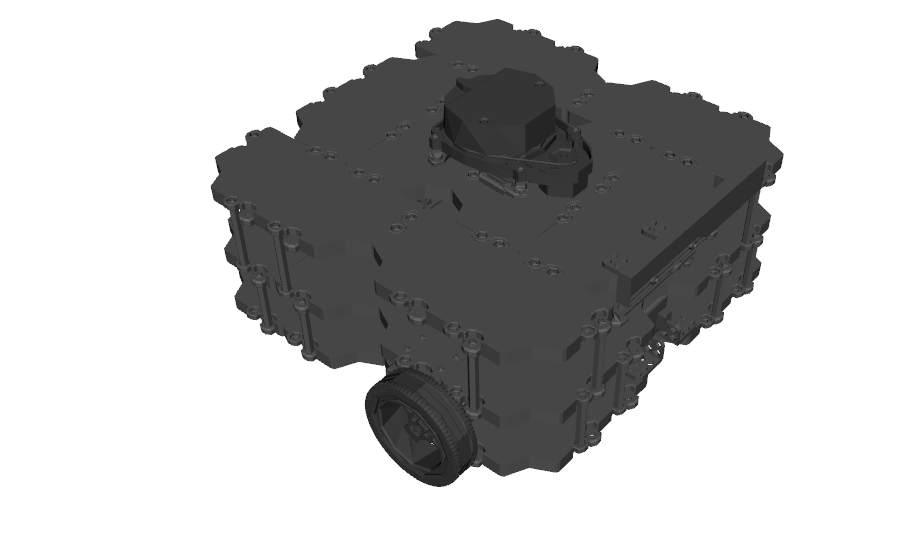
\includegraphics[width=1.0\textwidth]{images/turtlebot_sim.png}
	\caption{Turtlebot3 model in Gazebo simulator}
\end{figure}

The turtlebot will be used for the analysis of the current state of mobile navigation. Furthermore, the simulated turtlebot will be the plattform on which the behavior planning will be implemented and tested.

\subsection{ROS?!}
\textit{write sth about that?}

\subsection{Navigation2}
The ROS Navigation2 Stack (Nav2) is a combination of different packages that allows mobile robots to navigate from point A to point B. Navigation2 is the de-facto standard to achieve mobile navigation with a wide-range of supported robots. Supported robot types are holonomic, differential-drive, legged and ackerman (car-like). For the mobile robot to make use of the Nav2 stack, it has to be set up in a certain way to be able to generate plans and execute commands in the right way. Nav2 requires the mobile robot to possess a laserscan or pointcloud sensor, an odometry source (such as an IMU, wheel encoders) and a set of transformations to be available for planning and navigation. 
The stack contains tools that save and load occupancy maps, localize the robot, plan paths, execute the path, provide costmaps, build behaviors and execute recoveries \cite{macenski2020}. 

\begin{figure}[h!]
	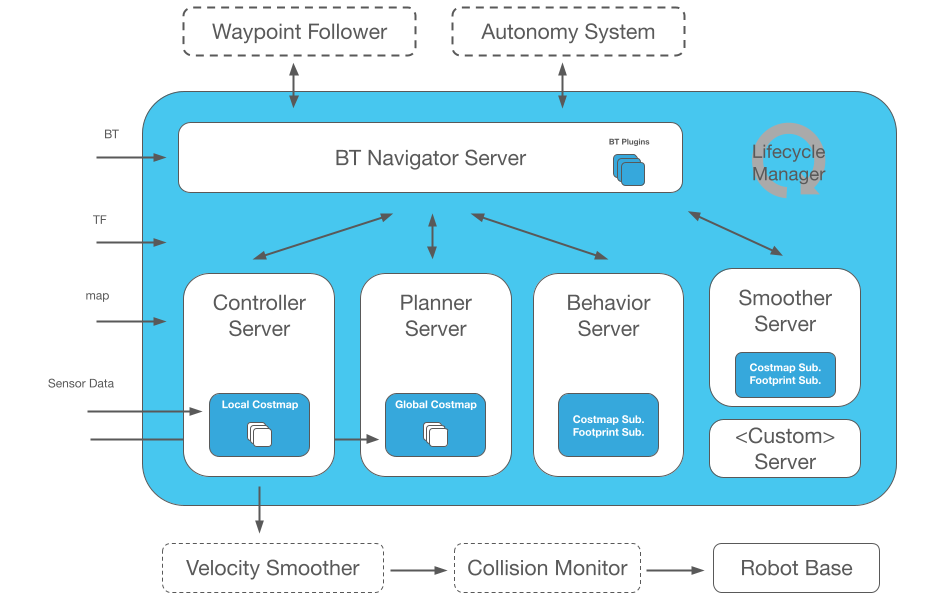
\includegraphics[width=1.0\textwidth]{images/nav2_architecture.png}
	\caption{Navigation2 Architecture \cite{macenski2020}}
\end{figure}
These packages are often combined with a SLAM method to build or enlarge maps. The path planning and path execution capabilities, which correspond to the global and local planner as described in section 2.2, are further supported by ready-to-use planning plugins which use A* and Dijkstra algorithms for path planning and a dynamic window approach for path execution. The system sequencing is done in a hierarchical structure as there is central behavior tree which calls asynchronous actions from the respective planners after another as seen in figure xx. 

\begin{figure} [h!]
	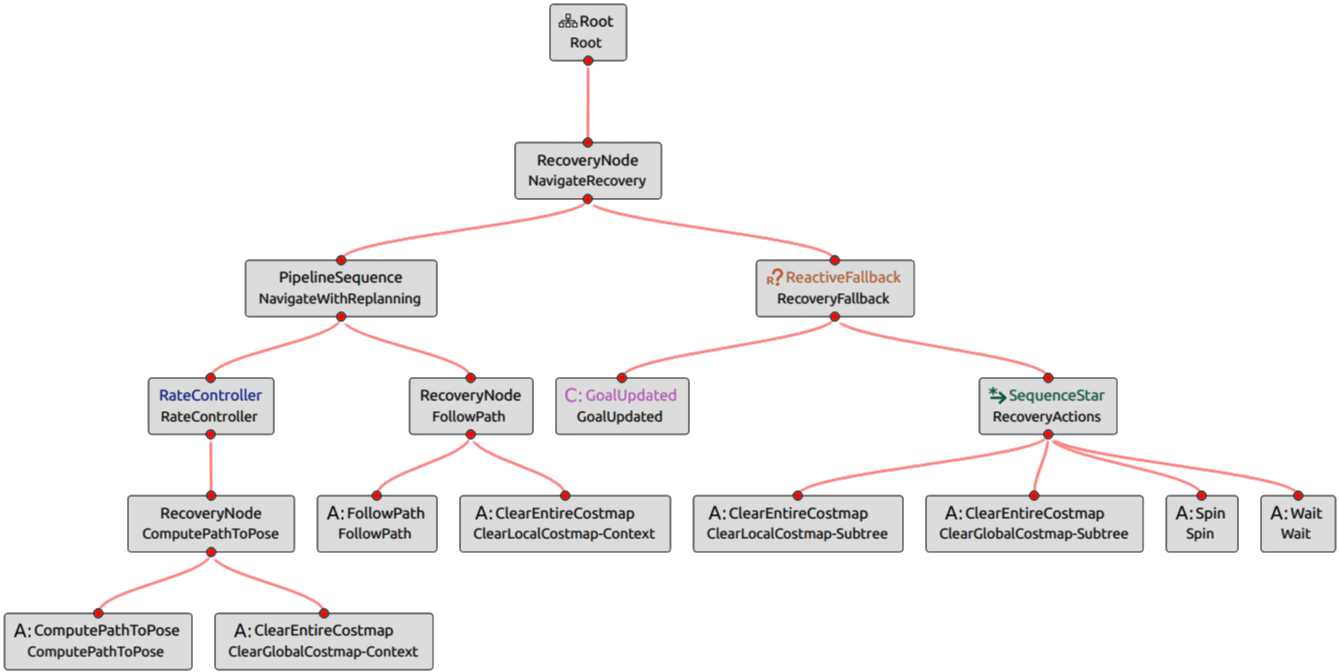
\includegraphics[width=1.0\textwidth]{images/nav_bt-modified.png}
	\caption{Navigation2 Behavior Tree}
\end{figure}

The behavior tree depicted in figure xx is the one that is the default Nav2 behvaior and has a set of recovery behaviors already implemented (spin, wait, backup, clear map). These behaviors are executed if the robot can not make progess towards the set goal. 
Nav2 makes use of a node lifecycle management system which is used to start, activate, deactivate and shutdown nodes in a controlled way. This allows the system degree to monitor the system's nodes startups, executions and failures. 

With this quantity of functions and hierarchical architecture the ROS Navigation2 stack is a great basis to achieve high levels of autonomy in robots. Due to the expandability of the software with plugins the software can be modified and expanded to fit the users needs. 
When comparing the functionalities of the software stack to the proposed autonomous system architecture in figure xx (2.2), the things that Nav2 are missing are a system-wide supervision layer and and a more deliberative approach to behavior planning as mentioned in 2.3.
The absence of these components leads to a limited set of circumstances in which the robot can perform navigation reliably. One of the core problems that behavior-based robots face is to generate a dependable environment representation as this is the basis for all of the latter steps in the planning part of the "Sense - Think - Act" cycle. Unforeseen events can severely limit the reliability of the environment representation without the robot being aware of it. Examples for such types of events that are currently not handled appropriatly are slipping wheels, orientation changes by external influences or undetected, more specifically undetectable obstacles. \textit{Add statistics about random sensor failures every ~10000h} This can lead for example to erratic movement of the robot, as reactive behaviors and more deliberative behaviors compete for authority over the robots movement. By design, in order to allow more intelligent robot behaviors, the deliberative behavior can override commands from reactive behaviors. But the deliberative behavior's planning is based upon a wrong representation of reality which then leads to unsafe commands which in turn triggers reactive-type behaviors again to counteract the commands from the deliberative behavior. Possibly the reactive behaviors do not get activated at all and the robot is continuing to drive despite being unaware of the surroundings. This would be a situation in which a human operator would need to step in and restore the robot to full functionality by hand. 

\textit{Add a closing statement about that suitability of the Nav stack for achieving autonomy}




\section{Risk Analysis For Requirement Prioritization}

\textit{Do that?}

\section{Requirements}

\textbf{How do I justify these requirements? Atm they are made arbitrarily with no real substance or reasoning.}

Functional Requirement List

number .. Name .. Description .. Success Criteria -.. Priority
freq1 Recovery The system can recover from crashes Ensure that the system can successfully reach goals despite previous crashes
freq2 Sensor Failure	The system detects sensor failures	Ensure that the system can restart sensors and decrease the speed during time sensor delivers limited information
freq3	Maintain operability The robot executes commands as long as it is safe	Ensure that the robot keeps driving if it is safe even when system functions are not working correctly
freq5	Emergency Detection	The system detects emergency. Ensure that the system can detect when the continuation on the calculated path is no longer safe (sensor failures, blockage)
freq6	Emergency Stop The system can initiate emergeny stops	Ensure that the system can override all commands and stop in case an emergency is detected
freq7	Override Navigation2 The system can override navigation2	Ensure that the system's commands can always override the commands coming from navigation2.
freq8 Reset Goals The system can reset and override goals set by the user so that the goal is reachable by planners.
freq9 Determinism The outcome for a given set of inputs has to be deterministic, meaning that the behavior is always executed in the same way. 

\begin{table}[h!]
\caption{Functional Requirements}
	\begin{tabular}{ | m{0.05\textwidth} | m{0.13\textwidth}| m{0.07\textwidth} | m{0.65\textwidth} |} 
  	\hline
  	Nr. & Name & Priority & Description \\ 
  	\hline
  	freq1 & Recovery & High &  The system can recover from crashes. Ensure that the system can successfully reach goals despite previous crashes\\ 
  	\hline
  	freq2 & Sensor Failure & High & The system detects sensor failure.Ensure that the system can restart sensors and decrease the speed during time sensor delivers limited information \\ 
  	\hline
  	freq3 & Maintain operability & High & The robot executes commands as long as it is safe	Ensure that the robot keeps driving if it is safe even when system functions are not working correctly \\
  	\hline
  	freq4 & Emergency Detection & High & The system detects emergency. Ensure that the system can detect when the continuation on the calculated path is no longer safe (sensor failures, blockage) \\
  	\hline
  	freq5 & Emergency Stop & High & The system can initiate emergeny stops. Ensure that the system can override all commands and stop in case an emergency is detected \\
  	\hline
  	freq6 & Override Navigation2 & High & The system can override navigation2. Ensure that the system's commands can always override the commands coming from navigation2. \\
  	\hline
  	freq7 & Reset Goals & Medium & The system can reset and override goals set by the user so that the goal is reachable by planners. \\
  	\hline
  	freq8 & Determinism & High & The outcome for a given set of inputs has to be deterministic, meaning that the behavior is always executed in the same way. \\
  	\hline
  	
  	
	\end{tabular}
\end{table}
Non-functional requirement list

number .. 	Name .. 				Description ..										Success Criteria
nfreq1 Single Point of Failure	The system does not have a single point of failure	When parts of the system fail the system maintains operability to a degree
nfreq2 Performance	The system's control loop guarantees fast reactions	The average frequence with which the system checks the sensors/navigation2 is higher than 100Hz (10ms)
nfreq3

\begin{table}[h!]
\caption{Non-Functional Requirements}
	\begin{tabular}{ | m{0.05\textwidth} | m{0.13\textwidth}| m{0.07\textwidth} | m{0.65\textwidth} |} 
  	\hline
  	Nr. & Name & Priority & Description \\ 
  	\hline
  	nfreq1 & Single Point of Failure & High &  The system does not have a single point of failure	When parts of the system fail the system maintains operability to a degree \\ 
  	\hline
  	nfreq2 & Performance & High & The system's control loop guarantees fast reactions. The average frequence with which the system checks the sensors/navigation2 is higher than 100Hz (10ms) \\ 
  	\hline
  	nfreq3 & Determinism & High & The outcome for a given set of inputs has to be deterministic, meaning that the behavior is always executed in the same way. \\
  	\hline
  	nfreq4 & Deliberate & High & The robot is able to execute deliberative behaviors, meaning that behaviors new implemented behaviors go beyond reacting to sensor input and have a planning aspect. \\
	\end{tabular}
\end{table}

\section{System Solution}

In order for a Turtlebot3 running Nav2 to appropriatly deal with the listed requirements, the system needs to be extended with new external modules. To eliminate a single point of failure for the system one needs to create an independent second system outside of the existing one. A suitable name for the second system is autonomy layer as it aims to increase the robustness and autonomy of the whole system. 
The autonomy layer provides a holistic system supervisor which monitors the health of all components (Sensors, Navigation, Robot Controller). This equips the system with the ability to deal with the event of node failures and component malfunctions. 
Another required addition to the autonomy layer is a data store of relevant system information. This not only includes sensor data, but also data like generated maps, costmaps, positions and speed commands. Making use of past datapoints allows behaviors to become more deliberative in their approach and opens up many possibilities for smart behaviors like movement predictions of obstacles. 
A third component to add to the autonomy layer is a behavior planner that is largely independent from the Nav2 execution and planning. This behavior planner 

\section{Software}

\subsection{Behaviortree.CPP}
The Navigation2 stack uses a behavior tree to coordinate the planning layer. The behavior tree that is used is an expansion of the Behaviortree.CPP (BT.CPP) library. This library offers a fast way to create, execute, monitor and edit behavior trees. 
Additionally to the types of control nodes that are mentioned in chapter 2.4.2 the library adds the concept of reactivity into the catalogue of control nodes. Reactive sequences and reactive fallbacks differ from normal ones in the handling of nodes that return the state "running". Instead of ticking the node again, the whole sequence restarts, which is very useful for continously checking a condition and executing an asynchronous action node, that gets halted when a condition is not met anymore. 

Also, it offers Decorator Nodes which allow more control over the child node and its output. These Decorator Nodes can only have one child node each. A comprehensive list of the available nodes and descriptions is in table xx.

\textit{TABLE HERE}

As a way to allow the tree nodes to communicate with each other, the library provides the developer with two possibilities. Either node can make use of the blackboard which is a dictionary (key/value) that all nodes of the tree can read and write. Or two nodes can be connected through ports which allows the direct communication between two nodes via a key/value.









 











